\documentclass[a4paper, 11pt, twosite, german, titlepage]{scrartcl}

%TODO doku
% German Support
\usepackage[german]{babel}
\usepackage[utf8]{inputenc}
\usepackage[T1]{fontenc}
% Math stuff
\usepackage{amsmath}
% style
\usepackage{fancyhdr}
\usepackage{newtxtext,newtxmath}
\usepackage[margin=2.5cm]{geometry}
% graphics
\usepackage{pgf, tikz}
\usetikzlibrary{decorations.pathreplacing, shapes}

%TODO Komaskript benutzen
% pagestyle: header...
\pagestyle{fancy}
\renewcommand{\sectionmark}[1]{%
\markboth {#1}{}}
\fancyhead[L]{Algebraische und kombinatorische Anwendungen in der Informatik SoSe16} 
\fancyhead[R]{\leftmark}	


%forall, exists, sum
\let\oldforall\forall
\renewcommand{\forall}{\hspace{3pt}\oldforall}
\let\oldexists\exists
\renewcommand{\exists}{\hspace{3pt}\oldexists}
\let\oldsum\sum
\renewcommand{\sum}{\oldsum\limits}
% Zahlbereiche
\DeclareMathOperator{\R}{\mathbb{R}}
\DeclareMathOperator{\Q}{\mathbb{Q}}
\DeclareMathOperator{\N}{\mathbb{N}}
\DeclareMathOperator{\Z}{\mathbb{Z}}
\DeclareMathOperator{\C}{\mathbb{C}}
% Zeichen
\newcommand{\gdw}{\Leftrightarrow} %iff (genau dann wenn)
\newcommand{\vnull}{\mathcal{O}} %Nullvektor
%
\newcommand{\ntoinf}{\stackrel{n \to \infty}{\longrightarrow}}
\newcommand{\inflimn}{\lim\limits_{n \to \infty}}
\newcommand{\inflimx}{\lim\limits_{x \to \infty}}
% Abk.
\newcommand{\without}[1]{\backslash \{#1\}} %Mengendifferenz
\newcommand{\abs}[1]{\left|#1\right|} % Betrag
\newcommand{\aset}[1]{\left\{#1\right\}} % Menge (grosse Klammern)
% 
\newcommand{\doubleunderline}[1]{\underline{\underline{#1}}}
\newcommand{\emphh}[1]{\textbf{#1}}








	
% Aufzaehlungsstandart		
\renewcommand{\labelenumi}{\alph{enumi})}

%TODO Titelseite
\title{Algebraische und kombinatorische Anwendungen in der Informatik}

% Dokumentinfo
\usepackage[pdftex, pdftitle={AKAI SoSe 16}, pdfauthor={Thomas Sachs, Felicia Saar}]{hyperref}
\hypersetup{pdftitle={AKAI}, pdfnewwindow, colorlinks, linkcolor=black}

\begin{document}

\maketitle
%TODO Disclaimer
\tableofcontents
\newpage
% muss hier zu Beginn stehen bleiben! Verhindert bei neuen Absaetzen das Einruecken
\setlength{\parindent}{0pt}
\setlength{\parskip}{1ex plus 0.5ex minus 0.2ex}


%Inhalt


\subsection*{Inhalt}
\begin{itemize}
	\item Abzählmethoden
	\item Rekursionen
	\item geordnete Mengen, Scheduling
	\item Anwendungen der linearen Algebra, z.B. Information Retrieval
\end{itemize}

\section{Abzählmethoden}

\subsection[Kardinalität paarweise disjunkter Mengen und des karthesischen Produkts]{} 
\label{subsec:disjcup(a)+kard(b)}
$S_1, \dots, S_n$ endliche Mengen
\begin{enumerate}
	\item  Sind $S_1, \dots, S_n$ paarweise disjunkt, so 
	\[\abs{S_1 \cup \dots \cup S_n} = \sum_{i=1}^{n}\abs{S_i}\]
	\item 
	\footnote{$S_1 \times \dots \times S_n = \aset{(s_1, \dots, s_n) : s_i \in S_i}$; Ist  $s_1 = s_2 = \dots = s_n = s  $ so $\underset{\leftarrow n \rightarrow}{s \times \dots \times s =: S^n}$}
	\[ \abs{S_1 \times \dots \times S_n} = \prod_{i=1}^n \abs{S_i} 
	 \]
\end{enumerate}

\subsection[Beispiel : Kardinalität der Vereinigung paarweise disjunkter Mengen]{Beispiele}

\begin{enumerate}
	\item
	Es gibt $2^n$ Wörter der Länge $n$ über $\aset{0,1}$
	\\ Allgemein Alphabet $S$ der Größe $q$, so gibt es $q^n$ Wörter der Länge $n$ über $S$
	
	\item[c)] Wie viele 3-stellige Zahlen (im Dezimalsystem; ggf. mit führenden Nullen) gibt es, die mindestens eine $1$ enthalten?
	Dafür gibt es mehrere\textbf{} Möglichkeiten:
	\begin{enumerate} %TODO Zahlen  + Mögl.
		\item $S =$ Menge aller 3.st. Zahlen mit mindestens einer 1.
		
		$S_1 = \aset{s \in S : \text{ an erster Stelle von } s \text{ steht } 1}$
		\\$S_2 = \aset{s \in S : \text{ die erste 1 von } s \text{ steht an 2. Stelle}}$
		\\$S_3 = \aset{s \in S : \text{ die erste 1 von } s \text{ steht an 3. Stelle}}$
		
		$S = S_1\: \dot{\cup}\; S_2 \;\dot{\cup}\; S_3$ 
		
		$S_1 = \aset{1} \times \aset{0, \dots, 9} \stackrel{\ref{subsec:disjcup(a)+kard(b)}b}{\Rightarrow} 
		\abs{S_1} = 1 \cdot 10 \cdot 10 = 100$
		\\
		$S_2 = \aset{0, 2, \dots, 9} \times \aset{1} \times \aset{0, \dots, 9} 
		\stackrel{\ref{subsec:disjcup(a)+kard(b)}b}{\Rightarrow} 
		\abs{S_2} = 9\cdot 1 \cdot 10 = 90$
		\\
		$S_3 = \aset{0, 2 \dots, 9} \times \aset{0, 2, \dots, 9} \times \aset{1}
		\stackrel{\ref{subsec:disjcup(a)+kard(b)}b}{\Rightarrow} 
		\abs{S_3} = 9 \cdot 9 \cdot 1 = 81$
		
		\ref{subsec:disjcup(a)+kard(b)}a: \quad 
		$\abs{S} = \abs{S_1} + \abs{S_2} + \abs{S_3} = 271$
		
		\item 
		$T_i = \aset{s \in S : s \text{ enthält mindestens } i \text{ mal die 1}}, i = 1, 2, 3, S = T_1 \;\dot{\cup}\; T_2 \;\dot{\cup}\; T_3$ 
		
		\begin{itemize}		
		
		\item $T_1 = T_1^1 \;\dot{\cup}\; T_1^2 \;\dot{\cup}\; T_1^3$,
	    \; $T_i^j = \aset{s \in T_1 : 1 \text{ steht an Stelle } j}$
	   
	    $\abs{T_1^1} = \abs{T_1^2} = \abs{T_1^3} = 9 \cdot 9 \cdot 1 = 81, 
	    \quad \abs{T_1} = 3 \cdot 81 = 243$ (\ref{subsec:disjcup(a)+kard(b)}) 
	    
	    \item  $T_2 = T_2^1 \cup T_2^2 \cup T_2^3$, 
	    \; $T_2^j = \aset{s \in T_2 : \text{ an der Stelle } j \text{ steht keine 1}}$
	    
	    $\abs{T_2^1} = \abs{T_2^2} = \abs{T_2^3} = 9$
	    \quad $ \abs{T_2} = 3 \cdot 9 = 27$
	    
	   \item  $\abs{T_3} = 1$
	    
	    \end{itemize}
	    
	    $\abs{S} = \abs{T_1 } + \abs{T_2} + \abs{T_3} = 271$
	    
	    \item
	    $G = \aset{0, \dots, 9}^3, \abs{G} = 1000$
	    
	    $S = G \without{\underbrace{x \in G : x \text{ enthält keine 1}}_{\aset{0, 2, \dots 9}^3}}$
	    
	    $\abs{\aset{0, 2, \dots, 9}^3} \stackrel{\ref{subsec:disjcup(a)+kard(b)}b}{=} 
	    9 \cdot 9 \cdot 9 = 729$
	    
	    $\abs{S} = 1000 - 729 = 271$
	 		
	\end{enumerate}
	
\end{enumerate}

\subsection*{Techniken im Beispiel}
\begin{itemize}
	\item Zerlegen einer abzählbaren Menge in disjunkte Teilmengen
	\item Abzählen des Komplements
\end{itemize}

Wie lässt sich \ref{subsec:disjcup(a)+kard(b)}a 
verallgemeinern, falls die $S_i$ nicht notwendig disjunkt?

$n=2$ : \begin{tikzpicture}
	\draw (0,0) circle (.5cm) node[above]{$S_1$};
	\draw (.7,0) circle (.5cm) node[above]{$S_2$};	
\end{tikzpicture}
$\abs{S_1 \cup S_2} = \abs{S_1} + \abs{S_2} - \abs{S_1 \cap S_2}$

$n=3$ : \begin{tikzpicture}
	\draw (0,0) circle (.5cm) node[above]{$S_1$};
	\draw (.7,0) circle (.5cm) node[above]{$S_2$};
	\draw (.35,-0.7) circle (.5cm) node[below]{$S_3$};	
\end{tikzpicture}
$\abs{S_1 \cup S_2 \cup S_3} = \abs{S_1} + \abs{S_2} + \abs{S_3}
                             - \abs{S_1 \cap S_2} - \abs{S_1 \cap S_3} - \abs{S_2 \cap S_3}
                             + \abs{S_1 \cap S_2 \cap S_3}$
                             
Allgemein gilt:

\subsection{Einschließungs-Ausschließungsprinzip}
\label{subsec:einausschliessprinzip}

\[\abs{ S_1 \cup \dots \cup S_n} = \sum_{k=1}^n(-1)^{k+1} \sum_{1 \leq i_1 < i_2 < \dots < i_k \leq n}{\abs{S_{i_i} \cap \dots \cap S_{i_k}}} \]
(Beweis WHK, 2.32)

\subsection{Beispiel : Einschließungs-Ausschließungsprinzip}

\begin{enumerate}
	\item Wie viele 8-stellige Zahlen (Dezimalsystem, mit führenden Nullen) enthalten nicht alle ungerade Ziffern?
	
	$S =$ Menge aller 8-st. Zahlen.
	\\$S_i = \aset{s \in S : s \text{ enthält nicht } i}, i = 1, 3, 5, 7, 9 $
	
	$\abs{S_1 \cup S_3 \cup S_5 \cup S_7 \cup S_9}$
	
	\ref{subsec:einausschliessprinzip} anwenden 
	($n=5 $)
	
	\begin{tabular}{l@{ : }lllc}

	$k=1$ 
	& $\underset{=9^8}{\abs{S_1}}, \dots, \underset{=9^8}{\abs{S_9}}$
	&
	& $5 \cdot 9^8$ 
	& (+)\\
	
	
	$k=2$ 
	& $\underbrace{\abs{S_1 \cap S_3}}_{\text{8-st. ohne 1, ohne 3}} = 8^8$, entsprechend $\abs{S_1 \cap S_5}, \dots \abs{S_7 \cap S_9}$ 
	& 10 mal 
	& $10 \cdot 8^8$ 
	&(-) \\
	
	$k=3$ 
	& $\abs{S_1 \cap S_3 \cap S_5} = 7^8$ 
	& 10 mal 
	&$10 \cdot 7^8$ 
	&(+) \\
	
 	$k=4$
 	& $\abs{S_1 \cap S_3 \cap S_5 \cap S_7} = 6^8$ 
 	& 5 mal 
 	& $5 \cdot 6^8$ 
 	& (-) \\
 	
 	$k=5$ 
 	& $\abs{S_1 \cap S_3 \cap S_5 \cap S_7 \cap S_9} = 5^8$ 
 	& 1 mal 
 	& $5^8$ 
 	& (+) \\
	 \end{tabular}
 		
	
	$\abs{S_1 \cup S_3 \cup S_5 \cup S_7 \cup S_9} = 5 \cdot 9^8 - 10 \cdot 8^8 + 10\cdot 7^8 - 5 \cdot 6^8 + 5^8 = 97.102.000$
	
		
	(ungefähr) $97\%$ aller 8-stell. Zahlen enthalten nicht alle ungeraden Ziffern.
		
	\item Wie lautet die Antwort in a), wenn man s-stelligen Zahlen ($s\geq 8$) betrachtet?\\	
	Wie in a): Anzahl $= 5*9^s-10*8^s+10*7^s-5*6^s+5^s$\\
		
	Anzahl aller s-stelligen Zahlen: $10^s$\\
		
	Verhältnis: $5*(\frac{9}{10})^s-10*(\frac{8}{10})^s+10*(\frac{7}{10})^s-5*(\frac{6}{10})^s+(\frac{5}{5})^s$
		
	Anal.: $q^s \rightarrow 0,$ falls $s \rightarrow \inf$, $\abs{q}<1$
	$lim V_s = 0$
	$s\rightarrow \inf$  
\end{enumerate}
                             



















\subsection{Prinzip des doppelten Abzählens}
\label{subsec:doppAbzaehlPrinzip}

$A, B$ endliche Mengen.
$S \subseteq A \times B$

Für jedes $a \in A$ sei $n_a = \abs{\aset{b \in B : (a, b) \in S}}$
\\Für jedes $b \in B$ sei $m_b = \abs{\aset{a \in A : (a, b) \in S}}$

Dann \[ \sum_{a \in A}n_a = \sum_{b \in B} m_b = \abs{S} \]


\subsubsection*{Speziell}

Angenommen $n_a = n$ für alle $a \in A$ und $m_b = m$ für alle $b \in B$.
%
\[\abs{A}\cdot n = \abs{B} \cdot m \]

\subsection[Beispiel : Handshaking-Lemma]{Beispiel}
Gegeben endlicher Graph. 

Graph $G$: Menge von Knoten (Ecken, \emph{vertex}), Menge von Kanten (\emph{edge}), jede Kante hat zwei Endknoten.
%
$G$ sei ohne Schleifen.

Dann: Anzahl der Knoten, von denen eine ungerade Anzahl von Kanten ausgeht, ist gerade. (Handshaking - Lemma)

$V=$ Menge der Knoten
\\$E=$ Menge der Kanten
\\$S \subseteq V \times E = \aset{(v, e), v \in V, e \in E, v \text{ ist Endknoten von } e}$
\\$v \in V : n_v =$ Anzahl der Kanten, die von $v$ ausgehen ($n_v =$ Grad von $v$)

\ref{subsec:doppAbzaehlPrinzip} : 
$\abs{S} = \sum_{v\in V} n_v = \sum_{e \in E} 2 = 2 \abs{E}$

$V = V_g \;\dot{\cup}\; V_u$,
\\$v \in V_g \gdw n_v$ gerade,
$v \in V_u \gdw n_v$ ungerade

$\sum_{v\in V_u}n_v + \sum_{v \in V_g}n_v = 2 \cdot \abs{E} \Rightarrow \sum_{v \in V_u}n_v$ gerade Zahl
$\Rightarrow \abs{V_u}$ ist gerade.

\subsection{Schubfachprinzip}
\label{subsec:schubfachprinzip}

Werden $m$ Objekte auf $n$ ''Schubfächer'' verteilt, so enthält (mind.) ein Schubfach mindestens $\left\lceil\frac{m}{n}\right\rceil$ Objekte. ($\lceil x \rceil = $ kleinste ganze Zahl $\geq x$)

\subsubsection*{Beweis}

$\left\lceil \frac{m}{n} \right\rceil - 1 < \frac{m}{n}$.
Angenommen Aussage ist falsch. D.h.. alle Schubfächer enthalten höchstens $\left\lceil \frac{m}{n} \right\rceil -1$ Objekte.

$\Rightarrow m \leq n \cdot \left(\left\lceil \frac{m}{n} \right\rceil -1\right) < n \cdot \frac{m}{n} = m $ %TODO lightning


\subsection[Beispiel: Anwendung Schubfachprinzip]{Beispiele} 

\begin{enumerate}
	\item Gegeben sein ein Quadrat der Seitenlänge 70cm. Kann man 50 Punkte so im Quadrat verteilen, dass je zwei Punkte mindestens Abstand von 15 cm haben?
	
	Zerlege das Quadrat in 49 Teilquadrate der Seitenlänge 10cm. Wenn man 50 Punkte im Quadrat verteilt, so enthält man nach \ref{subsec:schubfachprinzip} mindestens eines der kleinen Quadrate 2 Punkte.
	Maximalabstand in kleinem Quadrat ist durch die Diagonale gegeben, beträgt $\approx 14.14$ cm $< 15$ cm.
	
	\item
	Gegeben 6 Punkte in der Ebene, keine 3 auf einer Geraden. Je 2 Punkte durch Kante verbinden (vollst. Graph)
	
	Färbe Kanten in jeweils einer von 2 Farben (rot, grün).
	Dann gibt es ein einfarbiges Dreieck. 
	
	Gegeben sei irgendeine Färbung. Von den von einem Knoten $P$ ausgehenden 5 Kanten haben mindestens 3 die gleiche Farbe (\ref{subsec:schubfachprinzip}).
	
	Angenommen rote Kanten : $PQ, PR, PS$
	
	Falls $QR$ rot, so $PQR$ rotes Dreieck. O.B.d.A $QR$ grün.
	
	Analog: $QS$ und $RS$ o.B.d.A grün. Dann $QRS$ grün.
	
	\textbf{Spezialfall des Satzes von Ramsey (1930)}.
	
	Gegeben vollständiger Graph $G$ (alle Knoten sind durch Kanten verbunden).
	Färbe Knoten mit $f$ Farben. Wähle $r \in \N$
	
	Ist die Anzahl der Knoten von $G$ genügend groß, so existieren $r$ Knoten in $G$, so dass alle Kanten zwischen diesen $r$ Knoten die gleiche Farbei haben.
	(oben: $f=2, r=3$).
	
	(Beweis: Diekert, Kufsteiner, Rosenberger, Bd.1, Satz 6.29)
	
	
\end{enumerate}


\subsection*{Elementare Abzählprobleme (Mathe I)}

$n, k \in \N_0$

$[n]_0 := 1; k \geq 1: [n]_k := n \cdot (n-1) \cdot \dots \cdot (n-k + 1)$.
Für $k > n$ ist $[n]_k=0$

$[n]_n = n \cdot (n-1) \cdot 2 \cdot 1 = n!$ ($n$ Fakultät)

$\binom{n}{k} = \begin{cases}
	0 & k > n \\
	\frac{n!}{k!(n-k)!} & k \leq n
\end{cases} \;\;= \frac{[n]_k}{k!}$ Binomialkoeffizient.

$\binom{n}{k} = \binom{n}{n-k}$, $n, k \geq 1 : \binom{n}{k} = \binom{n-1}{k} + \binom{n-1}{k-1}$

$(a+b)^n = \sum_{k=0}^{n}\binom{n}{k}a^kb^{n-k} $ Binomialsatz.
\; Für $a=b=1$ : $ 2^n = \sum_{k=0}^{n}\binom{n}{k}  $ 
































\subsection{Satz}
\begin{enumerate}
\item $k,n \in \N_0$

Anzahl der Möglichkeiten aus einer Menge mit n Elementen \textit{k} Elemente auszuwählen ist:


\begin{tabular}{c|c|c}
	$k$ aus $n$ & ohne Berücksichtigung der Anordnung & mit Berücksichtigung der Anordnung\\ \hline
	ohne Wdhl. & $\binom{n}{k}$ & $[n]_k$\\ \hline
	mit Wdhl. & $\binom{n+k-1}{k} $& $n^k$
\end{tabular}


\item $k,n \in \N$

Anzahl der geordneten n-Tupel$(x_1,...,x_n)$

$x_i\in \N_0,$ mit $\sum_{i=1}^{n} = k$ ist $\binom{n+k-1}{k}$

\item $k,n \in \N$

Wie b), aber $x_i \in \N$; Anzahl ist $\binom{k-1}{n-1}$

$ \Biggl( \sum_{i=1}^{n}(x_i-1)=k-n$ \quad Nach b): Anzahl $\binom{n+(k-n)-1}{k-n} = \binom{k-1}{k-n}=\binom{k-1}{k-1-(k-n)} = \binom{k-1}{n-1} \Biggr) $ 
\item Nach a): Anzahl der k-elementigen Teilmengen einer Menge mit \textit{n} Elementen ist $\binom{n}{k.}$

Anzahl aller Teilmengen einer Menge mit n Elementen:
$$ \sum_{k=0}^{n}\binom{n}{k}= (1+1)^n = 2^n$$ (Mathe I)
\end{enumerate}

\subsection{Beispiel}
%TODO Add Felis tex

\subsection{Satz}
Anzahl der Möglichkeiten k identische/unterschiedliche Objekte auf \textit{n} identische/unterschiedl. Kisten zu verteilen (Kisten dürfen leer bleiben):

\begin{tabular}{c|c|c}
	& \textit{n} ident. Kisten & \textit{n} untersch. Kisten \\ \hline
	\textit{k} ident. Obj. &$p_n(k)$ &$\binom{n+k-1}{k})$ \\ \hline
	\textit{k} untersch. Obj. & $\sum_{i=1}^{n} S(k,i)$&$n^k$ 
\end{tabular}

\subsection{Definition}
\begin{enumerate}
	\item \textit{A} Menge. \underline{Partition} von \textit{A}: $\{ A_1,...,A_r \},~ A_i \subseteq A~ A_i\cap A_j = \emptyset$ für $i\neq j$ und $A = A_1 \cup ... \cup A_r$ 
	\subsubsection*{Beispiel:}
	$\abs{A}= 4$, $r=2$
	
	$\{\{1\}, \{2,3,4\}\},~ \{\{2\}, \{1,3,4\}\}~ \{\{3\}, \{1,2,4\}~ \{\{4\}, \{1,2,3\}\}\}$
	$\{\{1,2\}, \{3,4\}\},~\{\{1,3\}, \{2,4\}\},~\{\{1,4\}, \{2,3\}\}$ 7 Partitionen in zwei Teilmengen.
	
	\item Anzahl aller Partitionen einer Menge mit \textit{k} Elementen in r Teilmengen = 
	
	$$S(k,r)$$
	\begin{center}
	(Stirlingzahl 2.Art) \qquad \qquad  (James Stirling, 1692-1770)
	\end{center}
	
	\item Anzahl aller Partitionen einer Menge mit \textit{k} Elementen:
	
	$$ B_k = \sum_{i=1}^{k} S(k,i) \qquad \underline{Bell-Zahlen}$$
	\begin{center}
		(E.T.Bell,1883-1960)
	\end{center}
	
	\item $P_t(k) = $ Anzahl der Zerlegungen von $k\in \N_0$ in r Summanden aus $\N_0$ ohne Berücksichtgung der Reihenfolge der Summanden.
	
	$=\abs{\{(x_1,...,x_r): x_i \in \N_0, x_1 \geq x_2 \geq ... \geq x_r, \sum_{i=1}^{r} x_i=k\}} $
	
	\begin{tabular}{c c c c c}
	\underline{\textbf{Partitionszahlen Beispiel:}}	&	$P_2(4)=3$:& 4+0 & $P_3(4)=4$	& 4+0+0 \\
												 	&  			& 3+1    &				& 3+1+0 \\
													&   		& 2+2 	 & 				& 2+2+0 \\ 
													& 			&		 &				& 2+1+1 \\
	\end{tabular}


\end{enumerate}

\subsection*{Beweis 1.11}
%TODO Add Felis tex

\subsection{Satz}%TODO Add Feli's Part
\subsection{Satz}
$\abs{A}=k, \abs{B}=n$

Anzahl aller surjektiven Abb. $A \rightarrow B$ ist $\sum_{j=0}^{n-1}(-1)^j \binom{n}{j}(n-j^k)$

\subsubsection*{Beweis:}
Sei $B = \{b_1,...,b_n  \}$

\textit{S} = Menge aller surj. Abb. $A \rightarrow B$,

\textit{T} = Menge aller Abb.  $A \rightarrow B$,

$T_i = \{\alpha: A \rightarrow B: b_i \notin \alpha (A)  \}, i=1,...n$

Dann $S=T\backslash(T_1\cup ... \cup T_n)$

$\abs{T} = n^k$. Zu berechnen: $\abs{T_1 \cup ... \cup T_n}$ Mit 1.3 %TODO ref

$T_i$ besteht aus allen Abb. $A\rightarrow B\backslash\{b_i\}$

$\abs{T_i} = \underbrace{=}_{a)} (n-1)$ mit $n= \binom{n}{1}$  Mögl. für i

i<j: $\abs{T_i \cap T_j} = (n-2)^k$ mit $\binom{n}{2}$ Mögl. für i,j

i<j<l: $\abs{T_i \cap T_j \cap T_kl} = (n-3)^k$ mit $\binom{n}{3}$ Mögl. für i,j,l

$\abs{T_1 \cup ...\cup T_n} = \sum_{j=1}^{n}(-1)^{j+1} \sum_{1\leq i_1<...<i_j\leq n}\abs{T_{i_1}\cap ... \cap T_{i_j}} = \sum_{j=1}^{n}(-1)^{j+1} \binom{n}{j}(n-j)^k$

$\abs{S}= \abs{T}-\abs{T_1 \cup ... \cup T_n}$

$= n^k-\sum_{j=1}^{n}(-1)^{j+1}\binom{n}{j}(n-j)^{k}$

$= n^k+\sum_{j=1}^{n}(-1)^{j}\binom{n}{j}(n-j)^{k}$

$= \sum_{j=0}^{n-1}(-1)^{j}\binom{n}{j}(n-j)^{k}$

\subsection{Korollar}%TODO Add Feli's Part
\subsection{Korollar}
\begin{enumerate}
	\item $\sum_{j=0}^{n-1}(-1)^j\binom{n}{j}(n-j)^n = n!$
	
	\item Ist $n>k$, so ist $\sum_{j=0}^{n-1}(-1)^j\binom{n}{j}(n-j)^k=0$
\end{enumerate}
\subsection{Satz}%TODO Add Feli's Part

\subsection{Satz}
Seien $n \in \N , k_1,...k_d \in \N_0,~ k_1+...+k_d=n $

Gegeben seien d verschiedene Sorten von Objekten, jeweils $k_i$ identische von Sorte $i, i=1,...,d$

Die Anzahl der Möglichkeiten diese $k_1+...+k_d = n$ Objekte auf n Plätzen anzuordnen, ist:

$$ \frac{n!}{k_1!*k_2!*...*k_d!}$$ 

\subsubsection*{Beweis:}
Wähle $k_1$, der n Plätze für Objekte vom Typ 1 aus $\binom{n}{k_1}$ Möglichkeiten

Wähle $k_2$, der übrigen $n-1$ für Objekte vom Typ 2 aus $\binom{n-1}{k_2}$ Möglichkeiten

Wähle $k_3$, der übrigen $n-2$ für Objekte vom Typ 3 aus $\binom{n-2}{k_3}$ Möglichkeiten


.

.

.


Das liefert: $\binom{n}{k_1}\binom{n-k_1}{k_2}...\binom{n-k_1-...k_d-1}{k_d} = \frac{n!}{k_1!(n-k_1)!}*\frac{(n-k_1)!}{k_1!(n-k_1-k_2)!}*\frac{(n-k_1)!}{k_2!(n-k_1-k_2)!}*...*\frac{(n-k_1-...-k{d-1})!}{k_d!((n-k_1-...-k{d})!)}) $

$= \frac{n!}{k_1!*k_2!*...*k_d!}$ Möglichkeiten.

\subsection{Definition}
Sei $n \in \N, k_1,...,k_d \in \N_0,~ k_1+...+k_d = n$

Der \underline{Multinomialkoeffizient} $\binom{n}{k_1,k_2,...,k_d}$ ist derfiniert durch

$$\binom{n}{k_1,k_2,...,k_d} := \frac{n!}{k_1!k_2!...k_d!} $$

Beachte: $\binom{n}{k} = \binom{n}{k,n-k}$

Bezeichnung stammt vom \underline{Multinomialsatz:}

$x_1,...,x_d \in \R,$ so $(x_1+...+x_d)^n= \sum_{k_i \in \N}\binom{n}{k_1,k_2,...,k_d}x_1^{k_1}x_2^{k_2}...x_d^{k_d}$

\section{Linerare Rekursion}
\subsection{Definition}
\begin{enumerate}
	\item Eine \underline{Rekursion} ist ein unendliches System von Gleichungen der Form
	
	\begin{itemize}
		\item[($*)$] $x_n = f_n(x_{n-1,x_1})$ für alle $n\geq \underbrace{n_0}_{fest} $
		
		($f_n$ ist berechenbare Funktion)
		
	\end{itemize}
	Bei Vorgabe von beliebiger \underline{Anfangswerten} $x_1 = a_1,...,x_{n_0-1}=a_{n_0-1}$ sind $ a_{n_0}= f_{n_0-1}( a_{n_0-1},...,a_{1}), a_{n_0+1}= f_{n_0+1}(a_{n_0},a_{n_0-1},...,a_{1}),...$ festgelegt.
	
	Jede Folge $(x_1,x_2,...)$ von Elementen aus $\R$(oder $\C$), die $(*)$ erfüllt, heißt Lösung der Rekursion.
	
	\subsubsection*{Beispiel:}
	x$_n= x_{n-1}^2+2x_{n-2}x_1$ für n$\geq$ 3
	
	Anfangswerte: $a_1=1,~ a_2=2$
	
	$a_3 = a_2^2+2a_1^2=6$
	
	$a_4 = a_3^2+2a_2a_1=40$
	
	\item Eine \underline{Rekursion k-ter Ordnung:}
	
	$x_n=f_n(x_{n-1},...,x_{n-k}) $ für alle $n\geq k+1$
	
	\item Eine Rekursion heißt \underline{linear von Ordnung k mit sonstanten Koeffizienten}, falls
	
	$x_n= c_1x_{n-1}+c_2x_{n-2}+...+c_kx_{n-k} +g(n)$ für alle $ n\geq k+1$
	
	$c_1,...,c_k \in \R $(oder $\C$) fest (unabhängig von n), $c_k \neq 0$
	
	Ist $g(n)=0$ für alle $n\geq k+1$, so heißt Rekursion \underline{homogen}, ansonsten \underline{inhomogen}. 
	
\end{enumerate}

\subsection{Beispiel}
\begin{enumerate}
	\item \underline{Fibonacci-Zahlen}
	
	(Leonardo von Pisa $(*1170 ; \dagger1250$, Liber abaci)
	
	Auf wie viele Arten lässt sich $n \in \N$ als geordnete Summe von Eines und Zweien schreiben?
	
	
	\begin{tabular}{c c c}
		Anzahl $F_n$:	& $F_1=1$ 	& $1$\\
						& $f_2=2$	& $1+1,2$\\
						& $f_3=3$	& $1+1+1,1+2,2+1$\\
	\end{tabular}
	
	\begin{tabular}{c c l}
		$n\geq 3:$] 	&$\underbrace{+...+}_{n-1}+1$ & $F_n = F_{n-1}+F_{n-2}$, $F_1=1$, $F_2=2$\\
						&$\underbrace{+...++}_{n-2}+2$ &$F_4 = F_3+F_2 = 5$\\
						&								& lineare Rekursion mit konst. Koeff. Ordnung. 2, homogen 
	\end{tabular}
	\subsection*{Anderes Beispiel}
	Wie viele $0-1-$Folgen der Länge $n$ gibt es ohne zwei aueinanderfolgende Nullen?
	
	$a_1=2, a_2=3$
	
	$n\geq 3:$ $\overbrace{.......}^{a_{n-1}}1$ $a_n = a_{n-1}+a_{n-2}$ Fibonacci-Rekursion \quad $a_n=F_{n+1}$
	
	\qquad \quad $\overbrace{.......}^{a_{n-2}}10$
	 
	 
	 \item \underline{Türme von Hanoi}
	 \begin{center}
		 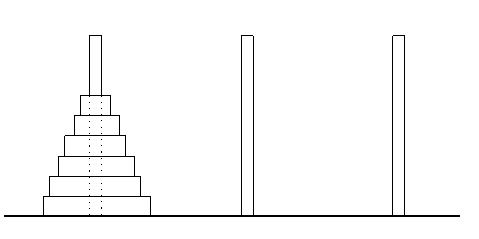
\includegraphics{hanoi.jpg}
	 \end{center}

	 3 Stäbe, n verschieden große Scheiben, auf Stab 1, der Größe nach geordnet, größte unten.
	 
	 Scheiben auf Stab 2 legen, in derselben Anordnung.
	 \begin{itemize}
	 	\item In jedem Zug 1 Scheibe umlegen
	 	\item Nie darf größere Scheibe auf kleinerer liegen
	 \end{itemize}
	 $a_n$ = Mindestanzahl von Zügen Stab 1 $\rightarrow$ Stab 2
	 
	 $a_1$ = 1
	 
	 obere $n-1$ Scheiben von Stab 1 $\rightarrow$ Stab 3 $\Rightarrow$ $a_n-1$ 
	 
	 größte Scheibe von Stab 1 $\rightarrow$ Stab 2 $\Rightarrow$ 1 
	 
	 alle Scheiben von Stab 3 $\rightarrow$ Stab 2 $\Rightarrow$ $a_{n-1}$ 
	 
	 \framebox[1\width]{$a_n = 2a_{n-1}+1$}, $n\geq2, a_1 = 1$ 
	 
	 linear, Ordnung. 1, inhomogen
	 
	 \item Verallg. von b) Divide-and-Conquer-Algorithmen:
	 
	 Zerlege Problem mit Inputgröße n in a Teilprobleme kleinerer Größe, z.B. $n - 1$,
	 
	 Max. Aufwand: $T(n) = a*T(n-1)+g(n)$
	 
	 
	 \qquad   \qquad \qquad \qquad  \qquad  \qquad \qquad \qquad$\Uparrow$

	 \qquad   \qquad \qquad  \qquad  \qquad \qquad \qquad Aufwand zum Zerlegen in Teilprobleme
	 
	 \qquad   \qquad \qquad  \qquad  \qquad \qquad \qquad und zum Zusammensetzen der Teillösungen
	 
	 \qquad   \qquad \qquad  \qquad  \qquad \qquad \qquad zur Gesamtlösung.
	 
	 
	 \item Bubble Sort
	 
	 Geg. Liste $(a_1, a_2, \dots, a_n)$ mit $n$ Elementen. Elemente seien paarweise vergleichbar bzgl $\leq$
	 Sortiere in absteigender Reihenfolge.
	 
	 Vergleiche $a_1, a_2$. Wenn $a_1 \geq a_2$ o.k. Wenn $a_1 \leq a_2$, so vertausche $a_1, a_2$.
	 
	 Fahre mit (dem neuen) $a_2$ fort. 
	% 
	 Am Ende steht das kleinste Element an der Stelle $n$. 
	 %
	 Rekursiv die ersten $n-1$ Elemente sortieren.
	 
	 Anzahl der Vergleiche : $V(n) = V(n-1) + \underbrace{(n-1)}_{g(n)}$
	 
	 lineare Rekursion der Ordnung 1, inhomogen, $g(n)$ ist nicht konstant.  
	 
	 
\end{enumerate}
$K = \R, \C$.
\\ geg. lineare Rekursion mit konstanten Koeffizienten der Ordnung $k$:
\[x_n = c_1x_{n-1} + \dots + c_kx_{n-k} + g(n)\] für alle $n \geq k +1$

Zu gegebenen Anfangswerten $(a_1, \dots, a_k) \in K^k$  existiert genau eine Lösung $(x_1, x_2, \dots) \in k^{\N}$ (= Menge aller unendlichen Folgen mit Einträgen aus $K$) mit $x_i = a_i$ für $1 \leq i \leq k$

$l : \begin{cases}
(a_1, \dots, a_k) \mapsto l(a) = \text{ Lösung mit Anfangswert } a_1, \dots, a_k \\ K1 k \to K^{\N}
\end{cases}$

\subsubsection*{Beispiel}

$x_n = 2x_{n-1} + 3x_{n-3}$, Ordnung 3, $(c_1 = 2, c_2 = 0, c_3 = 3)$

z.B. Anfangswerte $a=(0, 1, 2)$.
\\ $l(a) = (0, 1, 2, 4, 11, 28, 68, \dots)$

\subsection{Satz} %2.3
%TODO Thomas


Wunsch : Bringe $A$ auf Diagonalgestalt (d.h. finde Basis von $K^k$ aus Eigenvektoren zu $\alpha$!)

Bestimme Eigenwerte von $A$ (d.h. von $\alpha$). Charakteristisches Polynom $\det(t\cdot E_k - A)$ berechnen.

$\det(t E_k - A) = \det \begin{pmatrix}
t & -1 & & & &\\ 
&  t &-1  & & &\\
& & &\ddots  & & \\
& & & & t & -1 & \\
-c_k & -c_{k-1} & \cdot  && -c_2 & t -c_1 
\end{pmatrix}
= \footnote{Entwicklung nach der 1. Spalte}
\dots 
= t^k - c_1t^{k-1} - \dots - c_{k-1}t -c_k$

Eigenwerte von $A$ = Lösungen von
\[ t^k - c_1t^{k-1} - \cdot - c_{k-1}t - c_k = 0 \]

Sei $d$ eine Nullstelle des charakteristischen Polynoms, also Eigenwert von $A$.

Sei $\sigma \neq v = \begin{pmatrix}
v_1 \\ \vdots \\ v_k
\end{pmatrix}$ ein zugehöriger Eigenvektor. 

$\begin{pmatrix}
v_2 \\ \vdots \\ c_1v_k + \dots + c_kv_1
\end{pmatrix}
= Av
= dv
= \begin{pmatrix}
d \cdot v_1 \\ d \cdot v_2 \\ \vdots \\ d \cdot v_k
\end{pmatrix}
$\qquad
$\begin{array}{l}
v_2 = d \cdot v_1 \\
v_3 = d^2 \cdot v_1 \\
\vdots \\
v_k = d^{k-1}v_1
\end{array}$

Durch $v_1$ ist $v$ eindeutig bestimmt. Eigenraum von $\alpha$ zu Eigenwert $d$ ist 1-dimensional. Setze $v_1 = 1$

Eigenvektor zu $d$ : $v = \begin{pmatrix}
1 \\ d \\ d^2 \\ \vdots \\ d^{k-1}
\end{pmatrix}$

$v^t = (1, d, d^2, \dots, d^{k-1})$
\\$l(v^t) = (1, d, d^2, \dots, d^{k-1}, d^k, d^{k+1}, \dots) \in L$

$\begin{pmatrix}
v_{m-1} \\ \vdots \\ v_{m+k}
\end{pmatrix}
= A^m \begin{pmatrix}
v_1 \\\vdots\\v_k
\end{pmatrix}
= A^m \begin{pmatrix}
1 \\ d\\ \vdots \\d^{k-1}
\end{pmatrix}
= d^m \begin{pmatrix}
1 \\ d \\\vdots \\d^{k-1}
\end{pmatrix}
= \begin{pmatrix}
d^m \\ d^{m+1} \\\vdots \\d^{m+k-1}
\end{pmatrix}
$



















% TODO Thomas stuff

\subsection{Satz} % 2.4


Gegeben $(R_h) : x_n = c_1x_{n-1} + \dots + c_kx_{n-k}$ für $n > k$

\begin{enumerate}
	\item Ist $d\in\C$ eine Lösung der charakteristischen Gleichung 
	\[ (*) t^k - c_1t^{k-1} - \dots - c_{k-1}t - c_k = 0 \]
	so ist $w = (1, d, d^2, \dots)$ Lösung von $(R_h)$
	
	\item
	Besitzt (*) $k$ verschiedene Lösungen $d_1, \dots, d_k$, so bilden die $w_i = (1, d_i, d_i^2, \dots)$, $i = 1, \dots k$, Basis des Lösungsraums von $(R_h)$
	
	\item
	Unter den Vor. in b) sei $a = (a_1, \dots, a_k) \in \C^k$ ein Vektor von Anfangswerten.
	
	Seien $s_1, \dots, s_k$
 die Lösungen des LGS
 
	$\begin{array}{lcl}
	s_1 + \dots + s_k &=& a_1 \\
	d_1s_1 + \dots + d_ks_k &=& a_2 \\
	\vdots \\
	d_1^{k-1}s_1 + \dots + d_k^{k-1}s_k &=& a_k
	\end{array}$
	
	so ist $l(a) = (s_1 + \dots + s_k, s_1d_1 + \dots + s_kd_k, \dots, s_1d^{n-1} + \dots + s_kd_k^{n-1}, \dots)$

	d.h. \[ a_n = s_1d_1^{n-1} + \dots + s_kd_k^{n-1} \text{ für alle } n \in \N \]
	(\emph{geschlossene Form})
	
	
\end{enumerate}

\subsection{Beispiel} %2.5

\begin{enumerate}
	\item Fibonacci-Folge: 
	$F_n = F_{n-1} + F_{n-2}, n \geq 3, F_1 = 1, F_2 = 2$ (2.2.a) %TODO ref
	
	Charakteristische Gleichung 
	$t^2 - t - 1 = 0$
	\\ Lösungen : $d_{1,2} = \frac{1 \pm \sqrt{5}}{2}$
	
	$s_1 + s_2 = 1$
\\	$s_1\left(\frac{1 \pm \sqrt{5}}{2}\right) 
	+ s_2\left(\frac{1 - \sqrt{5}}{2}\right) = 2$
	
	$s_1 = \frac{1}{\sqrt{5}}\left(\frac{3 + \sqrt{5}}{2}\right)
	= \frac{1}{\sqrt{5}} \left( \frac{1 + \sqrt{5}}{2} \right)^2$
	\\ 
	$s_2= \frac{1}{\sqrt{5}} \left( \frac{-3 + \sqrt{5}}{2} \right) 
	= \frac{1}{\sqrt{5}} \left( \frac{1 - \sqrt{5}}{2} \right)^2$
	
	$F_n = s_1d_1^{n-1} + s_2d_2^{n-1}$
	%
	\[ F_n = \frac{1}{\sqrt{5}}\left( \frac{1 + \sqrt{5}}{2} \right)^{n+1} + \frac{1}{\sqrt{5}}\left( \frac{1 - \sqrt{5}}{2} \right)^{n+1} \]
	%
	(Manchmal wird auch definiert:
	$ F_n = \frac{1}{\sqrt{5}}\left( \frac{1 + \sqrt{5}}{2} \right)^n 
	+ \frac{1}{\sqrt{5}}\left(\frac{1 - \sqrt{5}}{2}\right)^n
	\\ F_1 = 1, F_2 = 1 $)
	 
	$\abs{\frac{1 - \sqrt{5}}{2}} < 1$, mit wachsendem $n$ geht $\frac{1}{\sqrt{5}}\left( \frac{1 - \sqrt{5}}{2} \right)^{n+1}$ gegen 0.
	
	Tatsächlich $F_n$ ist die nächste ganze Zahl zu $\frac{1}{\sqrt{5}}\left( \frac{1 + \sqrt{5}}{2} \right)^{n+1} \approx \frac{1}{\sqrt{5}}1.618^{n+1} $
	
	$\frac{1 + \sqrt{5}}{2}$ Zahl des goldenen Schnitts.
	
	$|---\underset{M}{-}---|--\underset{m}{-}--| \qquad \frac{M}{m} = \frac{M + m}{M} = \frac{1 + \sqrt{5}}{2}$
	
	
	\item 
	$x_n = 2x_{n-1} - x_{n-2} + 2x_{n-3}, n \geq 4, x_1 = 0, x_2 = 4, x_3 = 10 $

	$t^3 - 2t^2  + t - 2 = 0$
	\\ $d_1 = 2$
	\\ $t^3 - 2t^2 + t - 2 = (t-2)(t^2+1)$
	\\ $d_2 = i$, $d_3 = -i$
	

	$s_1 + s_2 + s_3 = 0$
	\\$2s_1 + is_2 - is_3 = 4$
	\\$4s_1 -s_2 -s_3 = 10$	
	
	$s_1 =2, s_2 = -1, s_3 = -1$
	
	$ x_n = 2 \cdot 2^{n-1} - i^{n-1} - (-i)^{n-1}
	      = \begin{cases}
	      2^n & n \text{ gerade} \\
	      2^n - 2 & n \equiv 1  \;(\!\!\!\!\mod 4) \\
	      2^n + 2 & n \equiv 3 \;(\!\!\!\!\mod 4)
	      \end{cases} $
	
	 

\end{enumerate}



\subsection{Satz} %2.6
%TODO Thomas stuff

\subsection{Beispiel} % 2.7

$x_n = 3x_{n-2} -2x_{n-3}, n \geq 4, x_1 = 1, x_2 = 2, x_3 = 6$

Charakteristische Gleichung $t^3-3t+2 = 0$, 
\\ $d_1 = 1$ (2 mal), $m_1 =2$
\\$t^3 -3t + 2 = (t-1)^2(t+2)$
\\$d_2 =2$ (1 mal), $m_2 = 1$

$w_{1,1} = (1, 1, 1, 1, \dots)$
\\ $w_{1, 2} = (1, 2, 3, 4, \dots)$
\\ $w_{2, 1} = (1, -2, 4, -8, \dots, (-2)^{n-1}, \dots)$

$(x_1, x_2, x_3, \dots) = s_1w_{1, 1} + s_2w_{1, 2} + s_3w_{2,1}$

$s_1 + s_2 + s_3 = 1$
\\$s_1 + 2s_2 -2s_3 = 2$ 
\\$s_1 + 3s_2 + 4s_3 = 6$

Lösung: $s_1 = - \frac{4}{3}, s_2 = 2, s_3 = \frac{1}{3}$

$x_n = -\frac{4}{3} + 2n + \frac{1}{3}(-2)^{n-1}$












































\end{document}